\documentclass[11pt]{beamer}
\usepackage{booktabs} 
\usepackage{graphicx}
\usepackage[utf8]{inputenc} 
\usepackage[russian]{babel} 
\usepackage{bm}
\usepackage{indentfirst}
\usepackage{amsfonts}
\usepackage{amsmath}
\usepackage{amsthm}
\usepackage{bbold}
\usepackage{moreverb}
\usepackage{dsfont}
\mode<presentation> {
	\usetheme{Warsaw}
	%\useinnertheme[shadow]{rounded}
	%\usecolortheme{wolverine}
	\usecolortheme{crane}
}

\DeclareMathOperator{\tr}{tr}
\DeclareMathOperator*{\argmin}{arg\,min}
\DeclareMathOperator*{\argmax}{arg\,max}

\newcommand*\oldmacro{}%
\let\oldmacro\insertshorttitle%
\renewcommand*\insertshorttitle{%
	\oldmacro\hfill%
	\insertframenumber\,/\,\inserttotalframenumber}
\newcommand{\RomanNumeralCaps}[1]
{\MakeUppercase{\romannumeral #1}}
\begin{document}
	\title[Классификация]{Обучение с учителем. Классификация. Дискриминантный анализ. Логистическая регрессия. Метод опорных векторов. Выбор модели с помощью кросс-валидации. Метод стохастического градиента}
	\author{Белкова Анна, Редкокош Кирилл, Лобанова Полина}
	
	\institute[] 
{
гр. 21.M03-мм \\
Санкт-Петербургский государственный университет \\
Кафедра статистического моделирования 
}

\begin{frame}
\titlepage 

\end{frame}

\begin{frame}{Метрики качества классификации. Матрица ошибок}
	Обсудим распространённые подходы к измерению качества моделей.
	
	Допустим, что у нас есть два класса и алгоритм, предсказывающий принадлежность каждого объекта одному из классов, тогда матрица ошибок классификации будет выглядеть следующим образом:
	
	\begin{table}[hhh]
		\begin{tabular}{|l|l|l|}
			\hline
			& y=1                 & y=0                 \\ \hline
			$\hat y = 1$ & True Positive (TP)  & False Positive (FP) \\ \hline
			$\hat y = 0$ & False Negative (FN) & True Negative (TN) \\ \hline
		\end{tabular}
	\end{table}
	
	Где $\hat y$ — это ответ алгоритма на объекте, а $y$ — истинная метка класса на этом объекте.
	Таким образом, ошибки классификации бывают двух видов: False Negative (FN) и False Positive (FP).
	
\end{frame}

\begin{frame}{Accuracy}
	Интуитивно понятной, очевидной и почти неиспользуемой метрикой является accuracy — доля правильных ответов алгоритма:
	
	\begin{align*}
		accuracy = \frac{TP + TN}{TP + TN + FP + FN}
	\end{align*}
	
	Эта метрика бесполезна в задачах с неравными классами, и это легко показать на примере.
	
\end{frame}

\begin{frame}{Precision, recall}
	
	Для оценки качества работы алгоритма на каждом из классов по отдельности введем метрики precision (точность) и recall (полнота).
	
	\begin{align*}
		precision = \frac{TP}{TP + FP}
	\end{align*}
	
	\begin{align*}
		recall = \frac{TP}{TP + FN}
	\end{align*}

	Precision можно интерпретировать как долю объектов, названных классификатором положительными и при этом действительно являющимися положительными, а recall показывает, какую долю объектов положительного класса из всех объектов положительного класса нашел алгоритм
	
\end{frame}

\begin{frame}{Precision, recall}
	\begin{figure}[hhh!]
		\begin{center}
			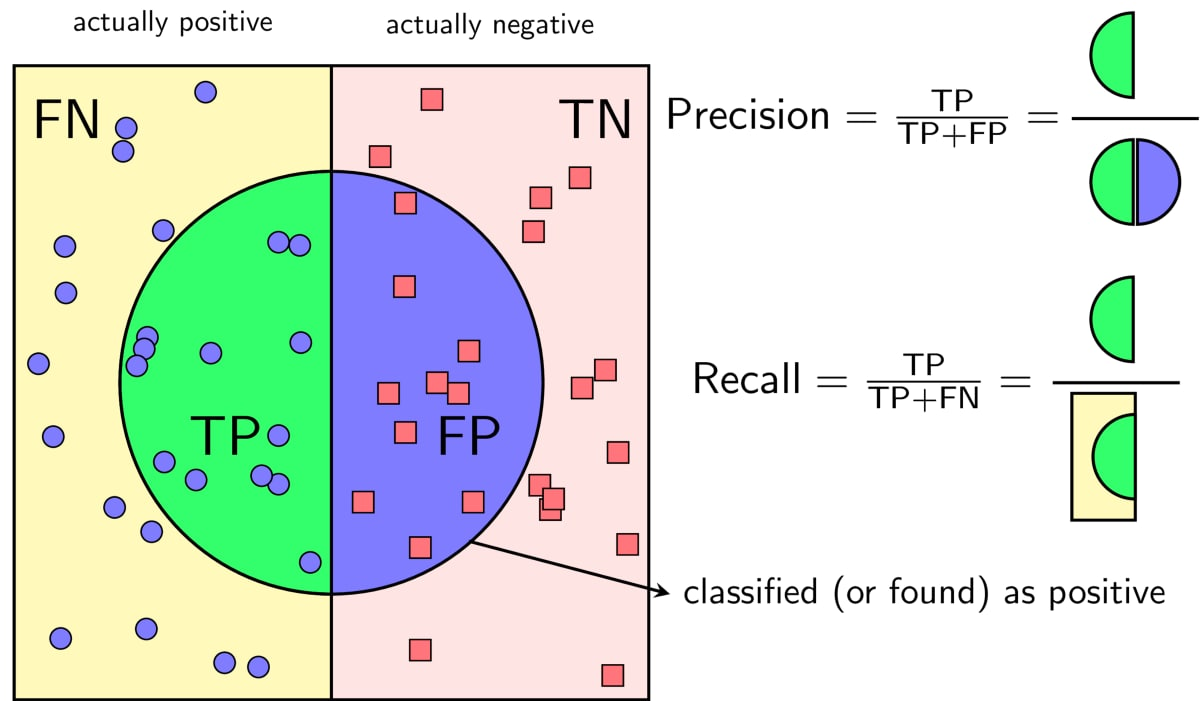
\includegraphics[width=9cm]{2022-10-06 01.03.42}
		\end{center}
		\vspace{-5mm}\caption{Precision, recall}
	\end{figure}
\end{frame}

\begin{frame}{F-мера}
Существует несколько различных способов объединить precision и recall в агрегированный критерий качества. F-мера (в общем случае $\ F_\beta$) — среднее гармоническое precision и recall :

\begin{align*}
	\ F_\beta = (1 + \beta^2) \cdot \frac{precision \cdot recall}{(\beta^2 \cdot precision) + recall}
\end{align*}

$\beta$ в данном случае определяет вес точности в метрике, и при $\beta = 1$ это среднее гармоническое (с множителем 2, чтобы в случае precision = 1 и recall = 1 иметь $\ F_1 = 1$)
F-мера достигает максимума при полноте и точности, равными единице, и близка к нулю, если один из аргументов близок к нулю.
\end{frame}

\begin{frame}{AUC-ROC}
	Одним из способов оценить модель, является AUC-ROC (или ROC AUC) — площадь (Area Under Curve) под кривой ошибок (Receiver Operating Characteristic curve ). Данная кривая представляет из себя линию от (0,0) до (1,1) в координатах True Positive Rate (TPR) и False Positive Rate (FPR):
	
	\begin{align*}
		TPR = \frac{TP}{TP + FN}
	\end{align*}	
	
	\begin{align*}
		FPR = \frac{FP}{FP + TN}
	\end{align*}

\end{frame}

\begin{frame}{AUC-ROC}
TPR-- это полнота, а FPR показывает, какую долю из объектов negative класса алгоритм предсказал неверно. В идеальном случае, когда классификатор не делает ошибок (FPR = 0, TPR = 1) мы получим площадь под кривой, равную единице; в противном случае, когда классификатор случайно выдает вероятности классов, AUC-ROC будет стремиться к 0.5, так как классификатор будет выдавать одинаковое количество TP и FP.
\end{frame}

\begin{frame}{AUC-ROC}
\begin{figure}[hhh!]
	\begin{center}
		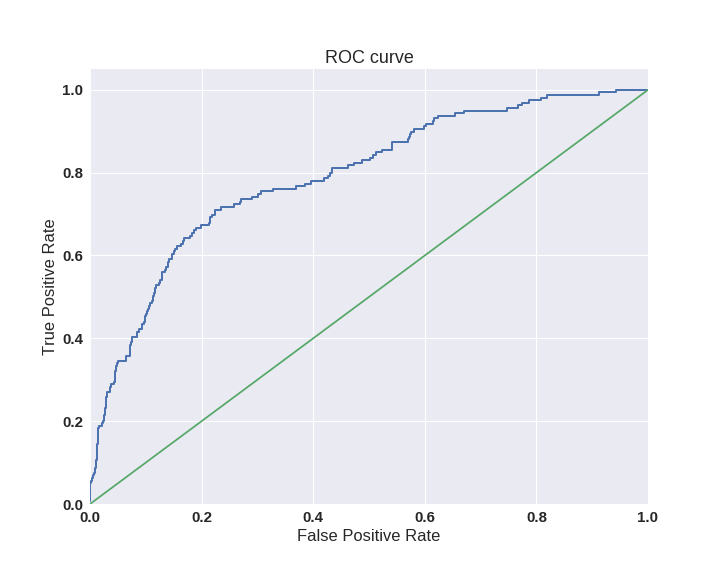
\includegraphics[width=9cm]{299157fad56a4ecca8f6b96b425bd38c}
	\end{center}
	\vspace{-5mm}\caption{ROC-кривая}
\end{figure}

\end{frame}

\begin{frame}{AUC-PR}
	Precision и recall также используют для построения кривой и, аналогично AUC-ROC, находят площадь под ней:
	
	\begin{figure}[hhh!]
		\begin{center}
			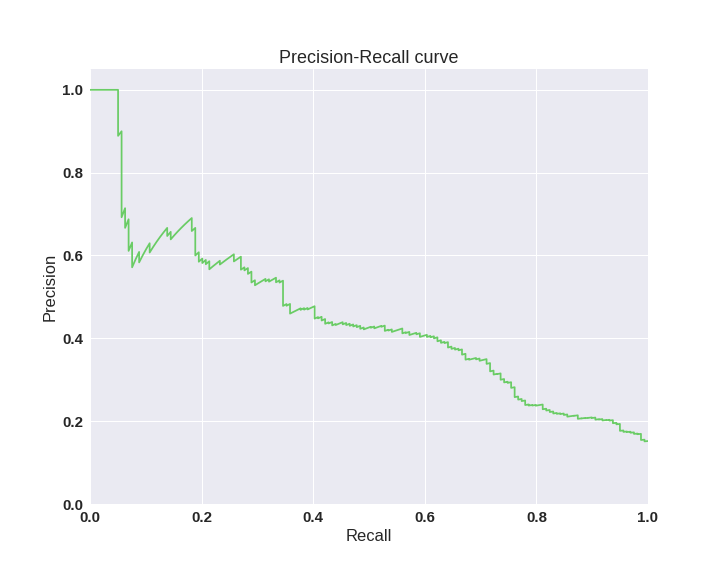
\includegraphics[width=7.5cm]{8873569147c24b49a2b7fa9ae883f20f}
		\end{center}
		\vspace{-5mm}\caption{PR-кривая}
	\end{figure}
\end{frame}

\begin{frame}{Модификации датасета для выравнивания соотношения классов}
	Одним из распространенных способов решения проблемы несбалансированных данных является избыточная выборка. Чрезмерная выборка относится к различным методам, которые направлены на увеличение количества экземпляров из недопредставленного класса в наборе данных.
	
	Самый простой способ сделать это - случайным образом выбрать наблюдения из класса меньшинства и добавить их в набор данных, пока мы не достигнем баланса между большинством и классом меньшинства. 
	
\end{frame}

\begin{frame}{(Synthetic Minority Over-sampling Technique, SMOTE)}
	\hfil\hfil\includegraphics[width=5cm]{0*2BcOfDa9avg5EsBv}\newline
	\null\hfil\hfil\makebox[5cm]{Step 1}\newline
	\vfil
	\hfil\hfil\includegraphics[width=5cm]{0*ESJbUSg6a0-nJE88}\hfil\hfil
	\includegraphics[width=5cm]{0*XvMdqBNsrjU5f8V5}\newline
	\null\hfil\hfil\makebox[5cm]{Step 2}
	\hfil\hfil\makebox[5cm]{Step 3}
\end{frame}

\begin{frame}{SMOTE Расширения}
	
	\begin{itemize}
		\item BorderlineSMOTE: Вместо избыточной выборки между всеми наблюдениями меньшинств, BorderlineSMOTE стремится увеличить количество наблюдений меньшинств, которые граничат с наблюдениями большинства. Цель здесь - дать классификатору возможность более четко различать эти пограничные наблюдения.
		\item SVMSMOTE: SVMSMOTE, как следует из его названия, использует алгоритм машины опорных векторов для генерации новых наблюдений меньшинства вблизи границы между классами большинства и меньшинства.
	\end{itemize}
	
\end{frame}

\begin{frame}{Tomek Links}
	
	\begin{figure}[hhh!]
		\begin{center}
			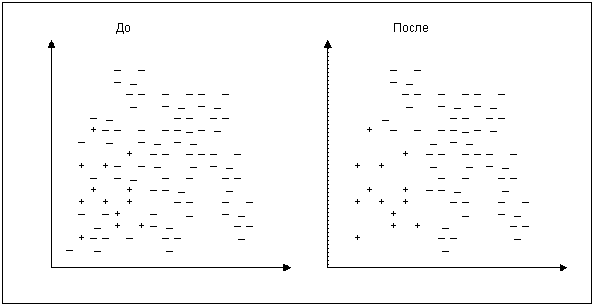
\includegraphics[width=10cm]{Tomek_links}
		\end{center}
		\vspace{-5mm}
	\end{figure}
	
\end{frame}


\begin{frame}{Дискриминантный анализ}
Суть дискриминантного анализа заключается в том, чтобы смоделировать распределение $X$ в каждом из классов отдельно, а затем использовать теорему Байеса, чтобы получить $P(Y = k \mid X = x)$.

\pause


Теорема Байеса:
\begin{align*}
	P(Y	= k \mid X = x) = \frac{P(X = x \mid Y = k) \cdot P(Y = k)}{P(X = x)}.
\end{align*}

\end{frame}

\begin{frame}{Байесовский классификатор}
	\bigskip
Для построения байесовского классификатора, нам необходимо знать апостериорные вероятности $P(Y \mid \xi = x)$.

Обозначим $p_i(x) = P(\xi = x \mid \eta =Y_i)$ условные плотности классов, $\pi_i = P(\eta = Y_i)$ -- априорные вероятности, $\sum_{i = 1}^{K} \pi_i = 1$. 

\pause
\bigskip
\bigskip
По теореме Байеса получим:
\begin{align*}
	P(Y = i \mid X = x) = \frac{p_i(x) \pi_i}{\sum_{i = 1}^K p_i(x)\pi_i}.
\end{align*}

Поэтому в качестве классифицирующих функций берут

$$f_i\left(x\right) = \mathrm P\left(x\middle\vert C_i\right) \pi_i = p_i(x) \pi_i.$$

\end{frame}

\begin{frame}{LDA}
	Предполагаем, что классы имеют нормальное распределение с одинаковой ковариационной матрицей. 
	
	Тогда плотность в точке $x$:
	
	$$p_i(x) = p\left(x\middle\vert \xi = Y_i\right) = \frac{1}{\left(2\pi\right)^{p/2}\left\vert\bm{\Sigma}\right\vert^{1/2}} \exp\left(-\frac{1}{2}{\left(x -\mu_i\right)^T}\bm{\Sigma}^{-1}\left(x -\mu_i\right)\right),$$
	
	\pause
	И классифицирующая функция $f_i\left(x\right) = \pi_i p\left(x\middle\vert \xi = Y_i\right)$, где $\pi_i$ --- априорная вероятность наблюдения попасть в $i$-ю группу. 
\end{frame}

\begin{frame}{LDA}
	
	Для упрощения вычислений можно переписать классифицирующую функцию через возрастающее монотонное преобразование как:
	
	$$g_i\left(x\right) = \log f_i\left(x\right) = \log \pi_i - \frac{1}{2}\log\left\vert\bm{\Sigma}\right\vert -  \frac{1}{2}{\left(x -\mu_i\right)^T}\bm{\Sigma}^{-1}\left(x -\mu_i\right).$$
	
	\pause
	
	Сократив часть, не зависящую от номера класса, получаем линейные классифицирующие функции:
	$$h_i(x) = -\frac{1}{2}{\bm{\mu}_i}^T\bm{\Sigma}^{-1}\bm{\mu}_i + {\bm{\mu}_i}^T\bm{\Sigma}^{-1}x + \log\pi_i.$$
	
\end{frame}

\begin{frame}{Канонические переменные}
	Задача: найти линейное преобразование $\mathbf{Z} = A^\mathrm{T}\mathbf X$, в результате которого получаются признаки наилучшим образом разделяющие группы. 
	
	\pause
	
	Вычислим внутриклассовую ковариационную матрицу:
	\begin{align*}
		\mathbf{E} = \frac{1}{n - K} \sum\limits_{i = 1}^K \sum_{j: y_j = Y_i} (x_j - \widehat{\mu}_i)^\mathrm{T}(x_j - \widehat{\mu}_i)
	\end{align*}
	Вычисляем межклассовую ковариационную матрицу (с точностью до коэффициента):
	\begin{align*}
		\mathbf{H} = \sum\limits_{i = 1}^K n_i (\widehat{\mu}_i - \widehat{\mu})^\mathrm{T}(\widehat{\mu}_i - \widehat{\mu}).
	\end{align*}
	
\end{frame}

\begin{frame}{Канонические переменные}
	Выборочная ковариационная матрица (с точностью до коэффициента) новых признаков имеет вид:
	\begin{align*}
		A^\mathrm{T}\mathbf{T}A = A^\mathrm{T}(\mathbf{E} + \mathbf{H})A = A^\mathrm{T}\mathbf{E}A + A^\mathrm{T}\mathbf{H}A,
	\end{align*}
	где $\mathbf{T}$ -- total covariance matrix, первое слагаемое -- оценка внутригрупповых отклонений, а второе -- оценка межгрупповых отклонений. Воспользовавшись критерием Фишера перейдем к обобщенной задаче на собственные числа и собственные вектора:
	\begin{align*}
		\frac{A^\mathrm{T}\mathbf{H}A}{A^\mathrm{T}\mathbf{E}A} \rightarrow \max_{A}.
	\end{align*}
\end{frame}

\begin{frame}{Канонические переменные}
Пусть $\lambda_1 \geq \lambda_2 \geq \ldots \geq \lambda_d$ -- собственные числа матрицы $\mathbf{E}^{-1}\mathbf{H}$, а $A_1, \ldots, A_d$ -- соответствующие им собственные вектора. Тогда максимум выше равен $\lambda_1$  и достигается на $A_1$. При этом $A^\mathrm{T}_i \mathbf{E}A_j = 0$. Далее
\begin{align*}
	\max_{A, A \bot A_1}\frac{A^\mathrm{T}\mathbf{H}A}{A^\mathrm{T}\mathbf{E}A} = \lambda_2,
\end{align*}
достигается на $A_2$ и так далее.

Вектора $A_i$ называют каноническими коэффициентами, а новые признаки $Z_i$ -- каноническими переменными, $Z_i$ ортогональны.
\end{frame}

\begin{frame}{Значимость канонических переменных}
	Возникает вопрос: сколько канонических переменных нам окажется достаточно взять? Другими словами, нужно проверить гипотезу:
	\begin{align*}
		H_0: A_i, i = \ell,\ldots,d~\text{не описывают отличия}.
	\end{align*}
\begin{itemize}
	\item Wilks' Lambda $$\Lambda_\ell^p = \prod_{i = l}^d \frac{1}{1 + \lambda_i};$$
	
	\item Roy's greatest root $$r_1^2 = \frac{\lambda_1}{1+\lambda_1};$$
	
	\item Pillai's trace $$V=trace(\mathbf H(\mathbf H + \mathbf E)^{-1});$$
	
	\item Hotelling-Lawley trace $$V=trace(\mathbf H \mathbf E^{-1}).$$
\end{itemize}
\end{frame}

\begin{frame}{QDA}
	Предполагаем, что каждый класс имеет многомерное нормальное распределение с различными ковариационными матрицами.
	
	\pause
	
	Тогда плотность в точке $x$
	$$p\left(x\middle\vert \xi = Y_i\right) = \frac{1}{\left(2\pi\right)^{p/2}\left\vert\bm{\Sigma}_i\right\vert^{1/2}} \exp\left(-\frac{1}{2}{\left(x -\mu_i\right)^T}\bm{\Sigma}_i^{-1}\left(x -\mu_i\right)\right),$$
	и классифицирующая функция $f_i\left(x\right) = \pi_i p\left(x\middle\vert \xi = Y_i\right)$. Применяем возрастающее монотонное преобразование и оставляем в классифицирующей функции только члены, отличающиеся в разных группах:
	
	$$g_i\left(x\right) = \log f_i\left(x\right) = \log \pi_i - \frac{1}{2}\log\left\vert\bm{\Sigma}_i\right\vert -  \frac{1}{2}{\left(x -\mu_i\right)^T}\bm{\Sigma}_i^{-1}\left(x -\mu_i\right),$$
	получаем квадратично зависящую от $x$ классифицирующую функцию.
\end{frame}

\begin{frame}{Наивный байесовский классификатор}
	Предположим, что признаки независимы внутри групп и имеют нормальное распределение:
	
	\pause
	
	\begin{align*}
		p_i(x) = \prod_{j = 1}^p p_{ij}(x_j), \quad p_{ij}(x_j) = \frac{1}{\sqrt{2\pi}\sigma_{ij}}e^{-\frac{(x_j -\mu_{ij})^2}{2\sigma^2_{ij}}}.
	\end{align*}
	Отсюда классифицирующую функцию можно представить в виде:
	\begin{align*}
		\delta_i(x) = -\frac{1}{2}\sum_{j = 1}^p\frac{(x_j -\mu_{ij})^2}{2\sigma^2_{ij}} + \log(\pi_i).
	\end{align*}
\end{frame}

\begin{frame}{Cross-validation}
	\begin{itemize}
		\item Имеется выборка ($X$, $Y$);
		
		\item Строим модель, зависящую от параметра $\theta$ и минимизирующую ошибку $J(X,Y; \theta, \lambda)$, где $\lambda$ --- параметр регуляризации. 
		
	\end{itemize}
	
	\pause
	
	Хотим подобрать такой параметр $\hat \theta$, чтобы минимизировать ошибку $J({X}_{new},{Y}_{new};\hat \theta,0)$ на новых индивидах.
	
	Вариант решения:
	\begin{itemize}
		\item Делим выборку ($X$, $Y$) случайным образом на три набора: (${X}_{train}$, ${Y}_{train}$), (${X}_{CV}$, ${Y}_{CV}$) и (${X}_{test}$, ${Y}_{test}$) ; 
		
		\item Перебираем набор параметров${\lambda_1,\ldots,\lambda_m}$; 
		
		\item Для каждого параметра $\lambda_i$ строим модель на ($\mathsf{X}_{train}$, ${Y}_{train}$) и считаем ошибку $J(X_{CV},Y_{CV};\theta_{i}, 0)$; 
		
		\item Берем $\lambda=\lambda_0$ c минимальной ошибкой (ему соответствует $\hat \theta$);
		
		\item Считаем ошибку модели $J(X_{test},Y_{test};\hat \theta,\lambda_0)$.
	\end{itemize}
\end{frame}

\begin{frame}{K-fold Cross-validation}
	Алгоритм:
	\begin{itemize}
		\item Делим выборку ($X$, $Y$) случайным образом на $K$ частей: (${X}_1$, ${Y}_1$),...,(${X}_K$, ${Y}_K$)  ; 
		
		\item Обозначим (${X}_k'$, ${Y}_k'$) набор, содержащий всех индивидов, кроме (${X}_k$, ${Y}_k$);
		
		\item Перебираем набор параметров ${\lambda_1,\ldots,\lambda_m}$; 
		
		\item Для каждого параметра $\lambda_i$ считаем: 
		$$
		CV_i=\sum_{j=1}^{K}\frac{n_j}{n} J({X}_j,{Y}_j;\theta_j,0),
		$$
		где $\theta_j$ минимизирует $J({X}_j',{Y}_j';\theta,\lambda_i)$, $n_j$ --- число индивидов в (${X}_j$, ${Y}_j$);
		
		\item Берем $\lambda=\lambda_0$ c минимальной ошибкой $CV_i$;
		
		\item Берем $\hat \theta$, которое минимизирует $J(X,Y;\theta,\lambda_0)$.
		
	\end{itemize}
\end{frame}

\end{document} 